\chapter{Proposed Coyote Integration}
\label{ch:coyote-integration}

\section{Integration Point}
\label{sec:coyote-integration-point}

The final goal is to place the bitstream checker directly on the Coyote deployment path. In this path, a user bitstream reaches the platform before partial reconfiguration. The checker should inspect the bitstream before it is loaded into the reconfigurable region.

Coyote provides a suitable target because it already separates platform services from user logic~\cite{korolija2020os,ramhorst2025coyote}. The static shell manages host communication, memory services, networking, command handling, and runtime control. User accelerators are deployed into reconfigurable regions. This structure gives a clear location for inspection before the partial reconfiguration step.

Figure~\ref{fig:coyote-integration} shows the proposed placement. The checker receives the user partial bitstream, applies preprocessing, runs the synthesized CNN, and returns a decision to the deployment logic.

\begin{figure}[t]
    \centering
    % Figure generated locally from figures/coyote_integration_path.dot.
    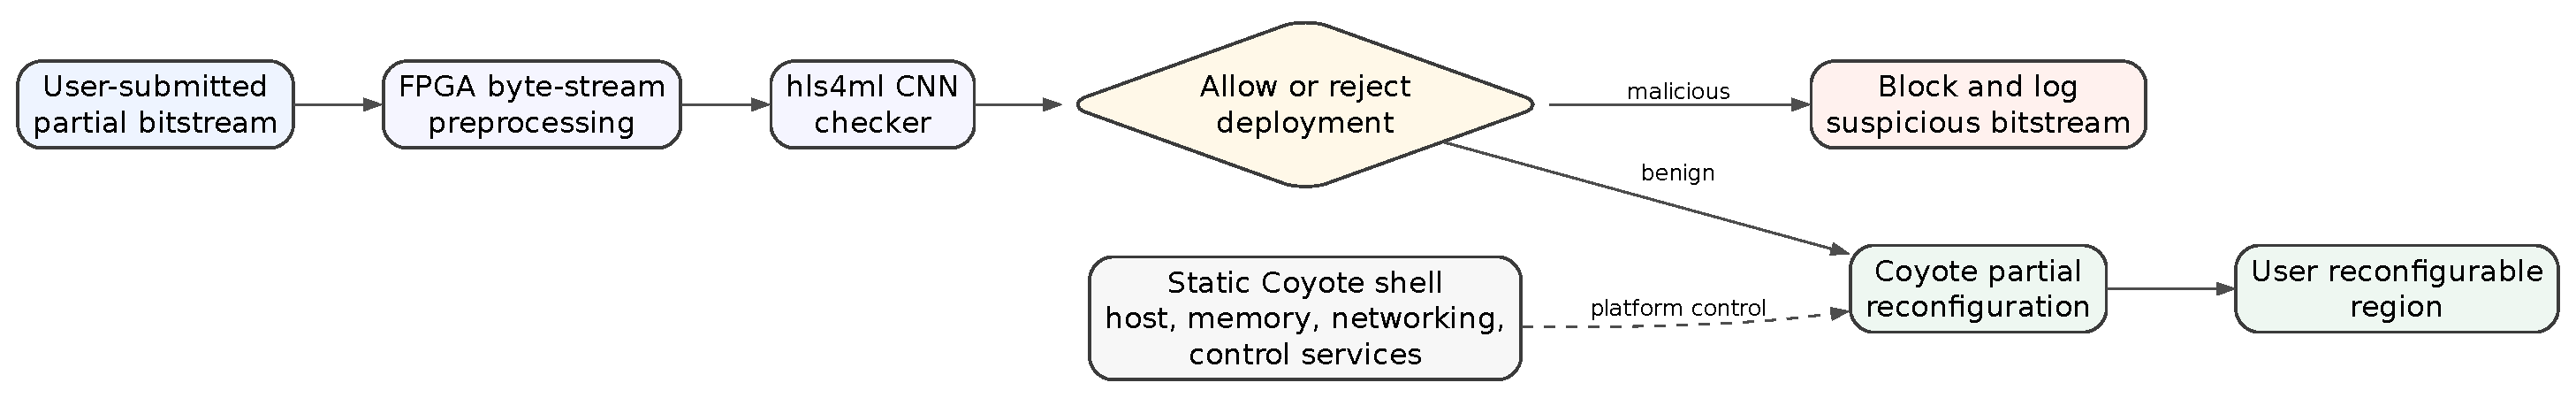
\includegraphics[width=0.95\linewidth]{figures/coyote_integration_path.pdf}
    \caption{Proposed Coyote integration path. The partial-bitstream checker is placed before partial reconfiguration and decides whether the bitstream should be loaded or rejected.}
    \label{fig:coyote-integration}
\end{figure}

\section{Checker Flow}
\label{sec:checker-flow}

The checker follows the same pipeline used during model evaluation. The incoming partial bitstream is treated as a byte stream. The preprocessing logic resizes the stream into the fixed tensor shape expected by the CNN. The synthesized hls4ml model then produces a maliciousness score or binary prediction.

The deployment logic uses this output to control partial reconfiguration. If the score is below the rejection threshold, the bitstream is allowed to continue to the PR controller. If the score is above the threshold, the platform blocks the reconfiguration and logs the event.

The intended flow is:

\begin{center}
\small
\begin{tabular}{c}
\textbf{user bitstream} $\rightarrow$ \textbf{preprocessing} $\rightarrow$ \textbf{CNN checker} \\[3pt]
$\rightarrow$ \textbf{allow or reject} $\rightarrow$ \textbf{partial reconfiguration}
\end{tabular}
\end{center}

This design keeps inspection inside the FPGA deployment path. It avoids a separate host-side inspection stage and gives the platform a self-contained gate before loading user logic. This follows the broader goal of making FPGA-resident ML components deployable inside systems paths rather than treating them only as offline models~\cite{heer2025ml4sys}.

\section{Prototype Scope}
\label{sec:coyote-prototype-scope}

This work evaluates the main components needed for such an integration. The preprocessing method has already been implemented as HLS C++ raw-byte downsampling logic, lowered to Verilog by the HLS flow, and used for the deployment-oriented latency results. The CNN candidates are synthesized with hls4ml and evaluated for latency and resource cost.

The current integration is still a proposal and prototype direction. A complete Coyote deployment would require control-plane integration, threshold policy, logging, error handling, and validation with the real PR controller. It would also need a clear policy for low-confidence predictions.
